\chapter{Convergence and Errors}
\label{AppendixB}

In this section a brief discussion on the convergence of the data and error calculus is done.

\section{Quantum Trajectories Method}
The QT method, explained in section~\ref{chapt3_qtm}, doing the stochastic unraveling of the master equation, builds the quantum trajectories after which it is named.  Every quantum trajectory corresponds to a simulated experiment and for the model under consideration, has an oscillatory profile as that displayed in fig.~\ref{fig:SS_s8J10511}. In order to stabilize the solution, for every quantum trajectory, the average in time is considered, starting from the end of the transient (needed for a solution of the Lindblad equation to converge towards the steady-state).

\begin{figure}[H]
    \centering
    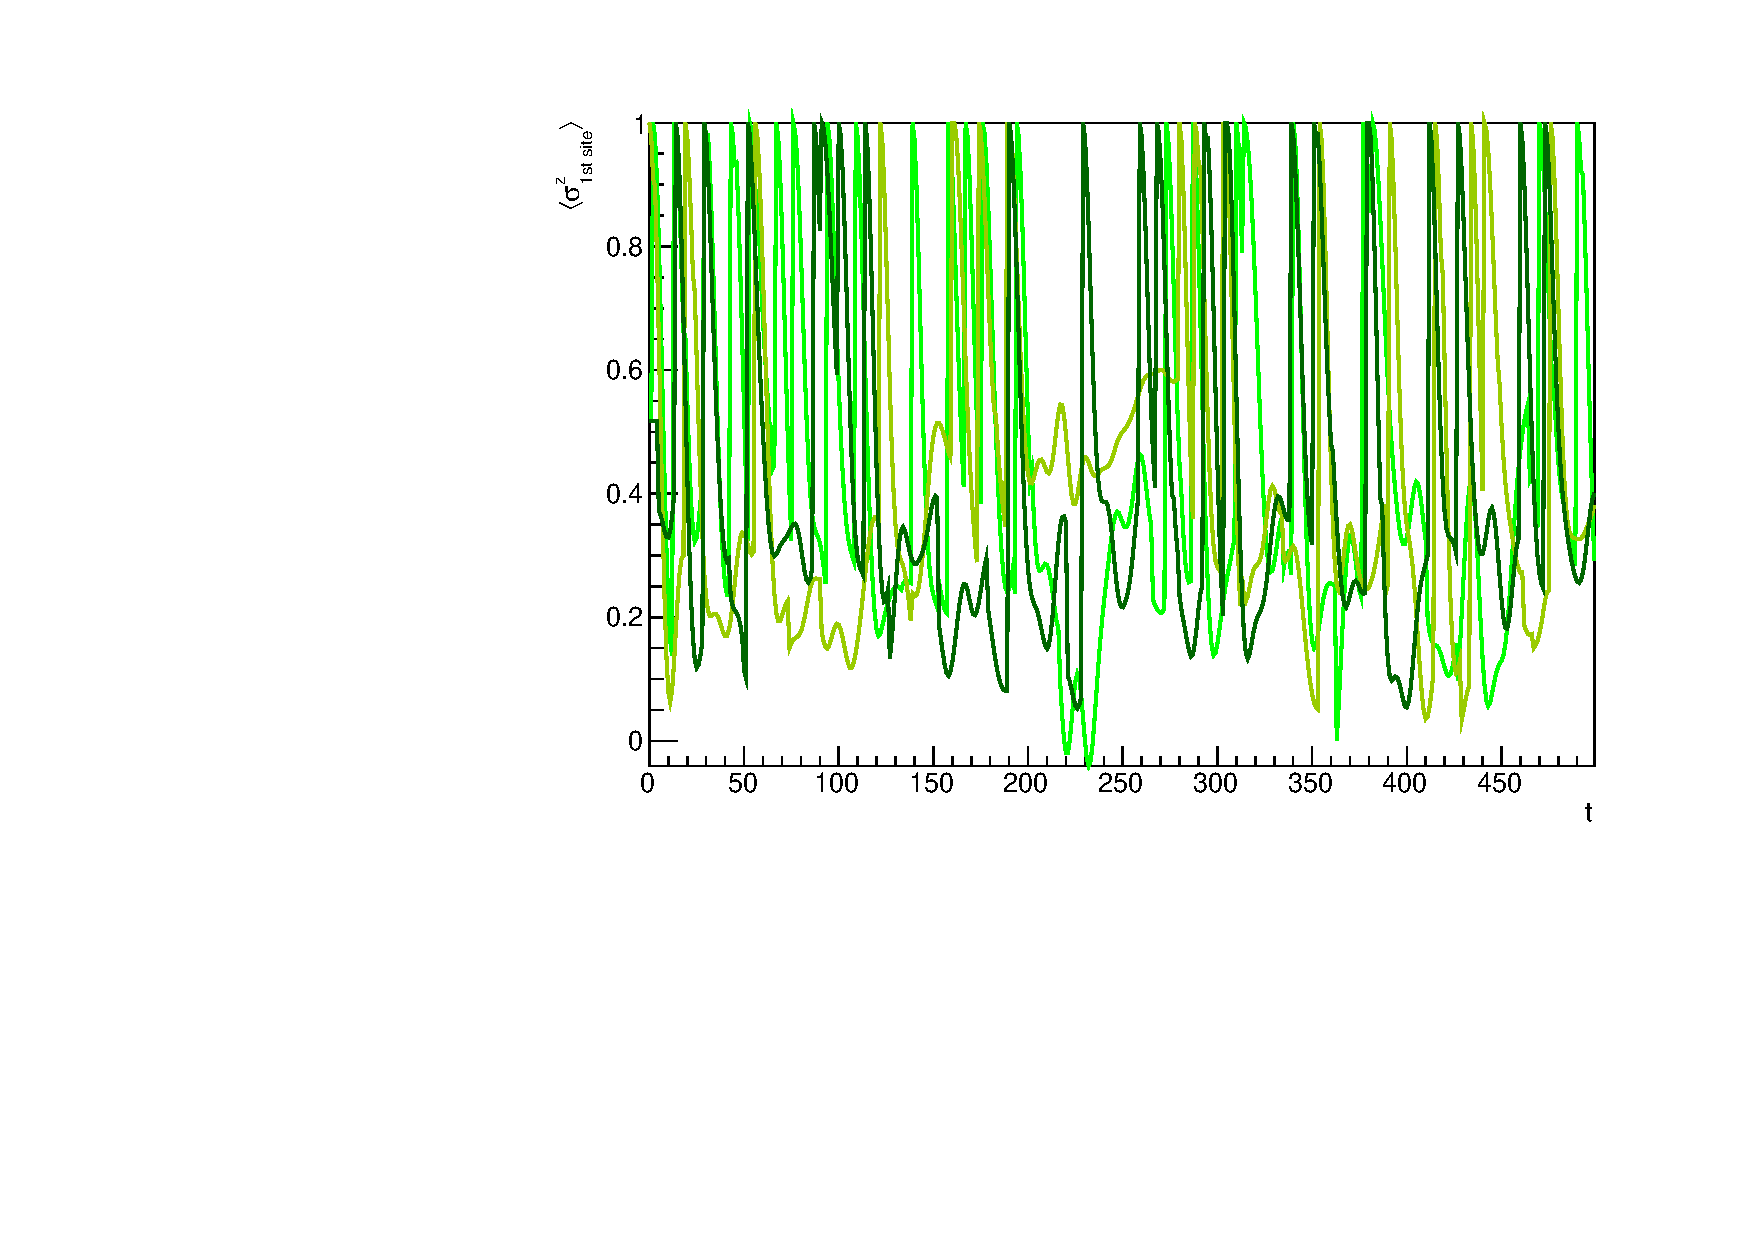
\includegraphics[scale=0.7]{Figures/QTrajectories3.pdf}
    \captionsetup{width=1.\linewidth}
    \caption{Example of three quantum trajectories; in particular, this is the expectation value of the magnetization of the first site of the chain, for $J_z = 1$ and $\gamma = 1$. The total elapsed time is $T=500$, while the time step $dt = 0.1$.}
    \label{fig:QTrajectories3}
\end{figure}

For the same case considered in fig.~\ref{fig:QTrajectories3}, the convergence of the mean values is shown in fig.~\ref{fig:Convergence_s8J1051}. 

\begin{figure}[H]
    \centering
    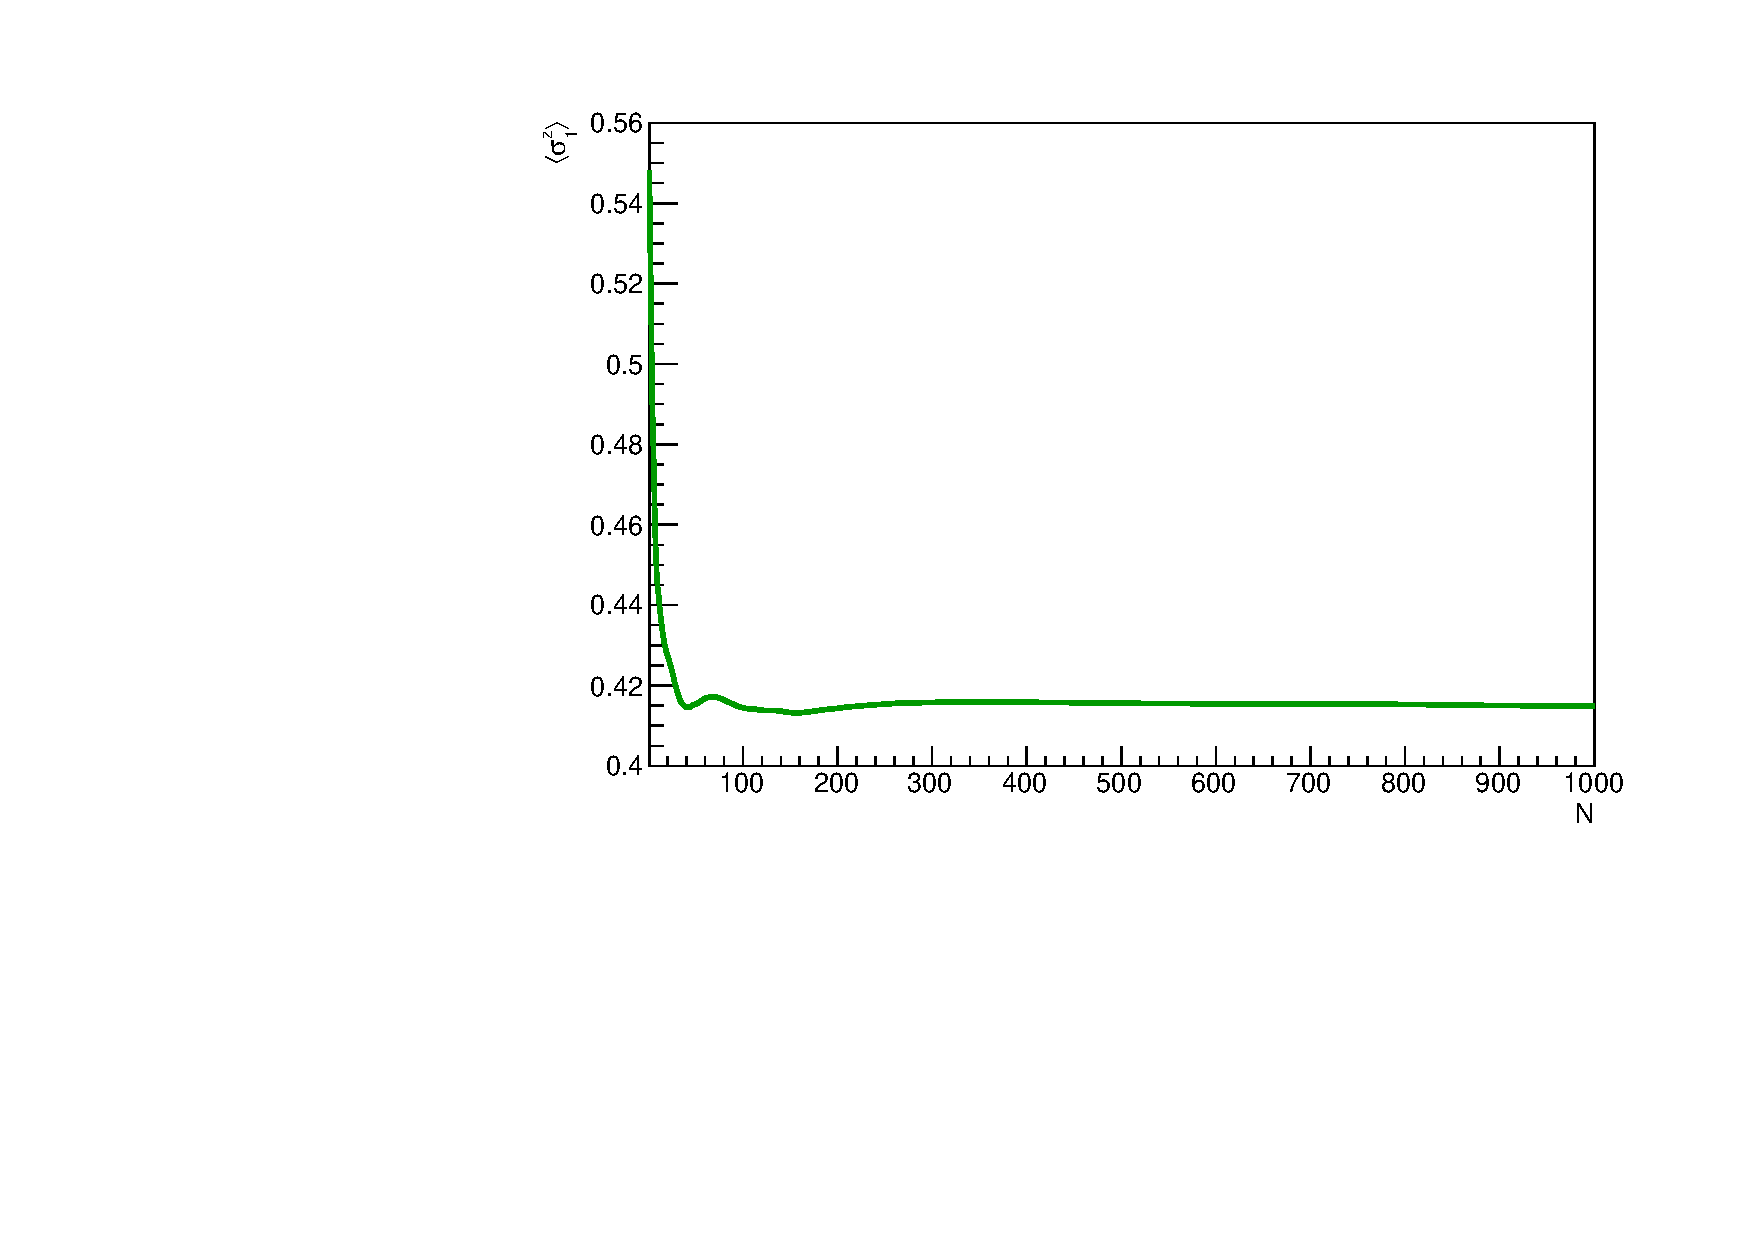
\includegraphics[scale=0.7]{Figures/Convergence_s8J1051.pdf}
    \captionsetup{width=1.\linewidth}
    \caption{Study of the convergence of the mean values of the quantum trajectories. For the case under consideration, the number of events is $N = 1000$.}
    \label{fig:Convergence_s8J1051}
\end{figure}

The study of the 8-sites chain was done with an elapsed time for every event of $T = 500$ and time-step $dt = 0.1$. The number of the simulated events is $N = 1000$.

As an error it has been consider the standard deviation of the mean, i.e.
\begin{equation*}
    \sigma_{\text{mean}} = \frac{\sigma}{\sqrt{N}},
\end{equation*}
where $\sigma$ is the standard deviation of the mean in time in the quantum trajectory.

\section{Matrix Product Density Operators Method}
The convergence of MPO method depends essentially on the setting of two parameters: the bond dimension and the number of Trotter steps. The fig.~\ref{fig:convergenceMPO_8sites} shows the convergence profile for a 8-sites chain for $J_z = 1$ and $\gamma = 1$. The same quantity can reach convergence in different times if, for example, $J_z$ assumes another value. 

In the present work, for 8-sites chain it was considered a bond dimension $m = 100$ and Trotter steps in the range $[1200, 1500]$; for 12-sites chain it was considered a bond dimension $m = 60$ and Trotter steps in the range $[1000, 2000]$; for 16-sites chain it was considered a bond dimension $m = 80, 100$ and Trotter steps in the range $[1000, 1500]$.

In fig.~\ref{fig:convergence_8_12_16} the convergence of $\sigma^z$ for the first site of 8, 12, 16-sites chains. 

\begin{figure}[H]
\centering
\begin{subfigure}{\columnwidth}
\centering
    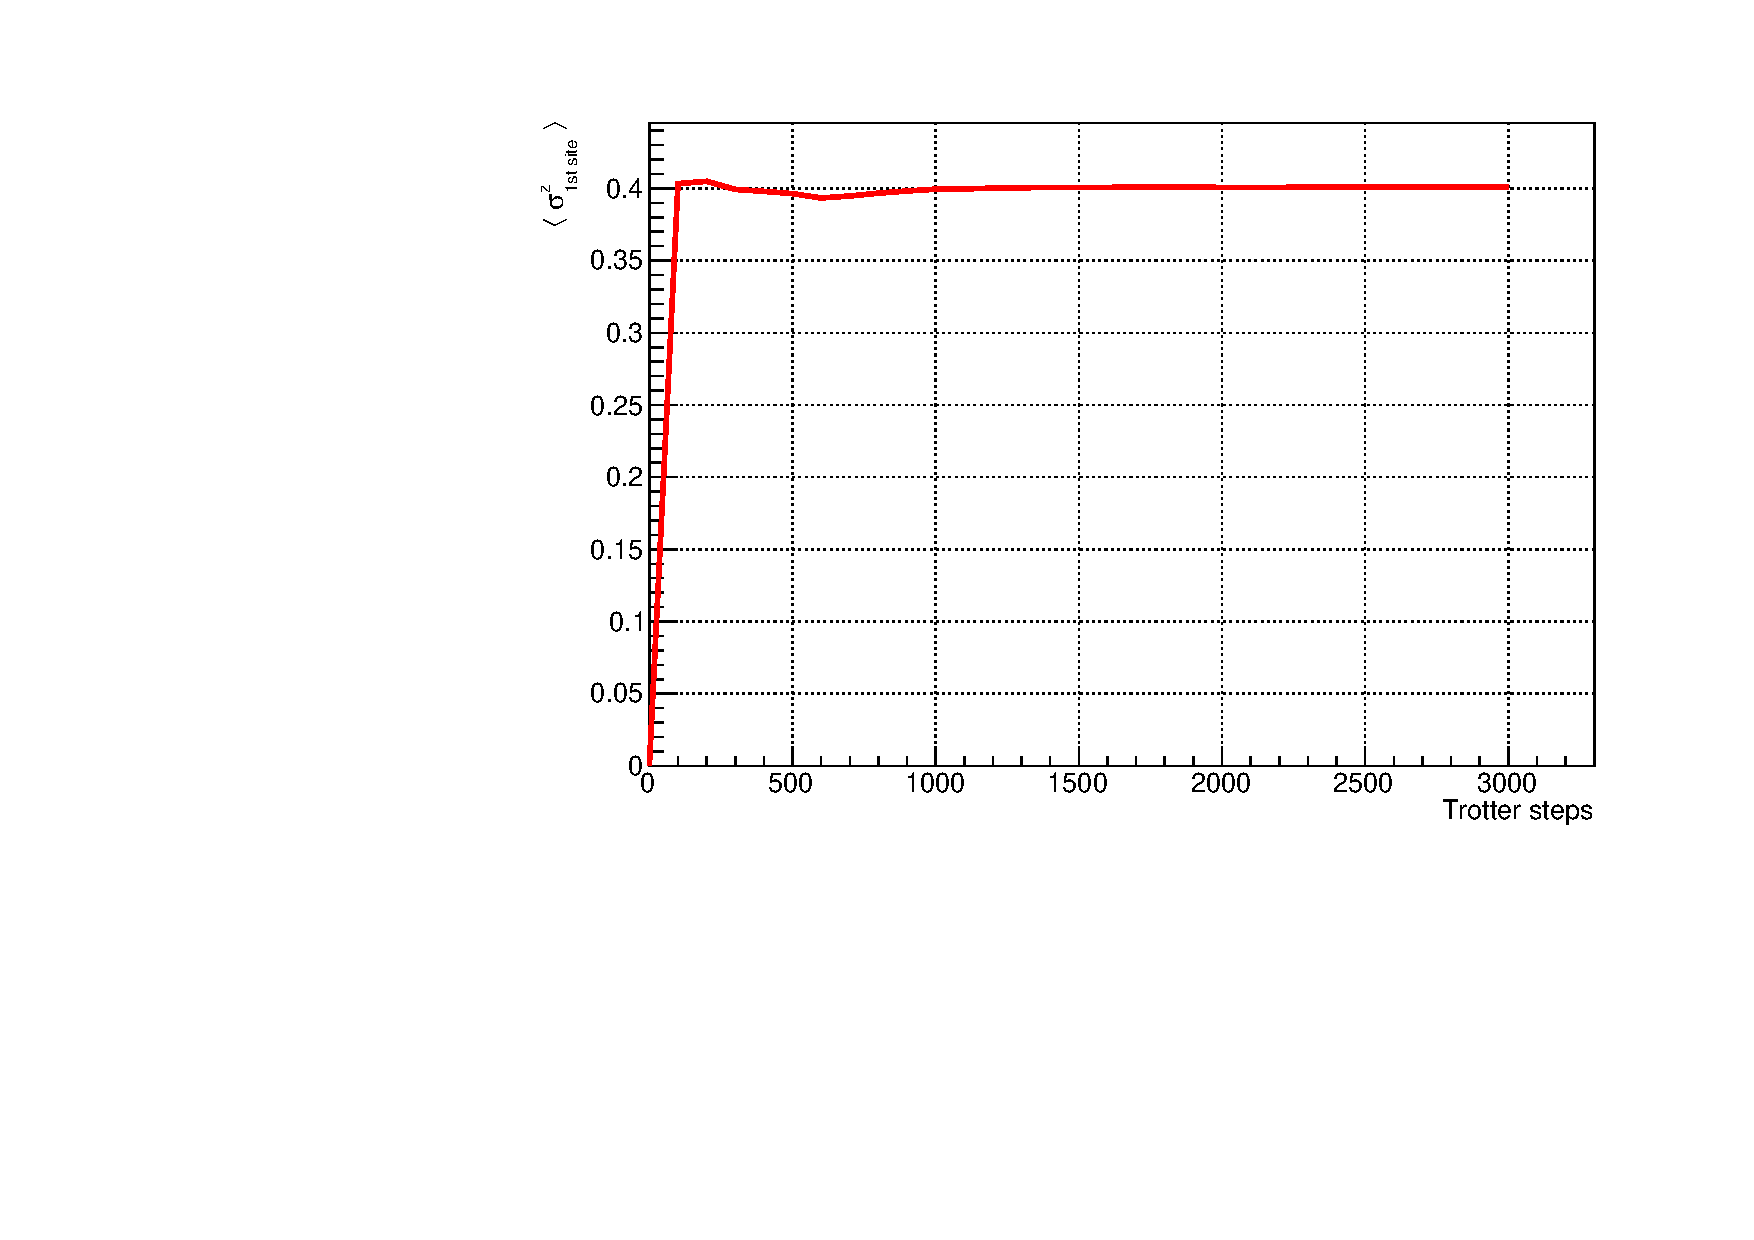
\includegraphics[scale=0.6]{Figures/convergence/Convergence_s8T3000J1051.pdf}
    \label{fig:8sites_LMvsGamma}
\end{subfigure}\quad
\begin{subfigure}{\columnwidth}
\centering
    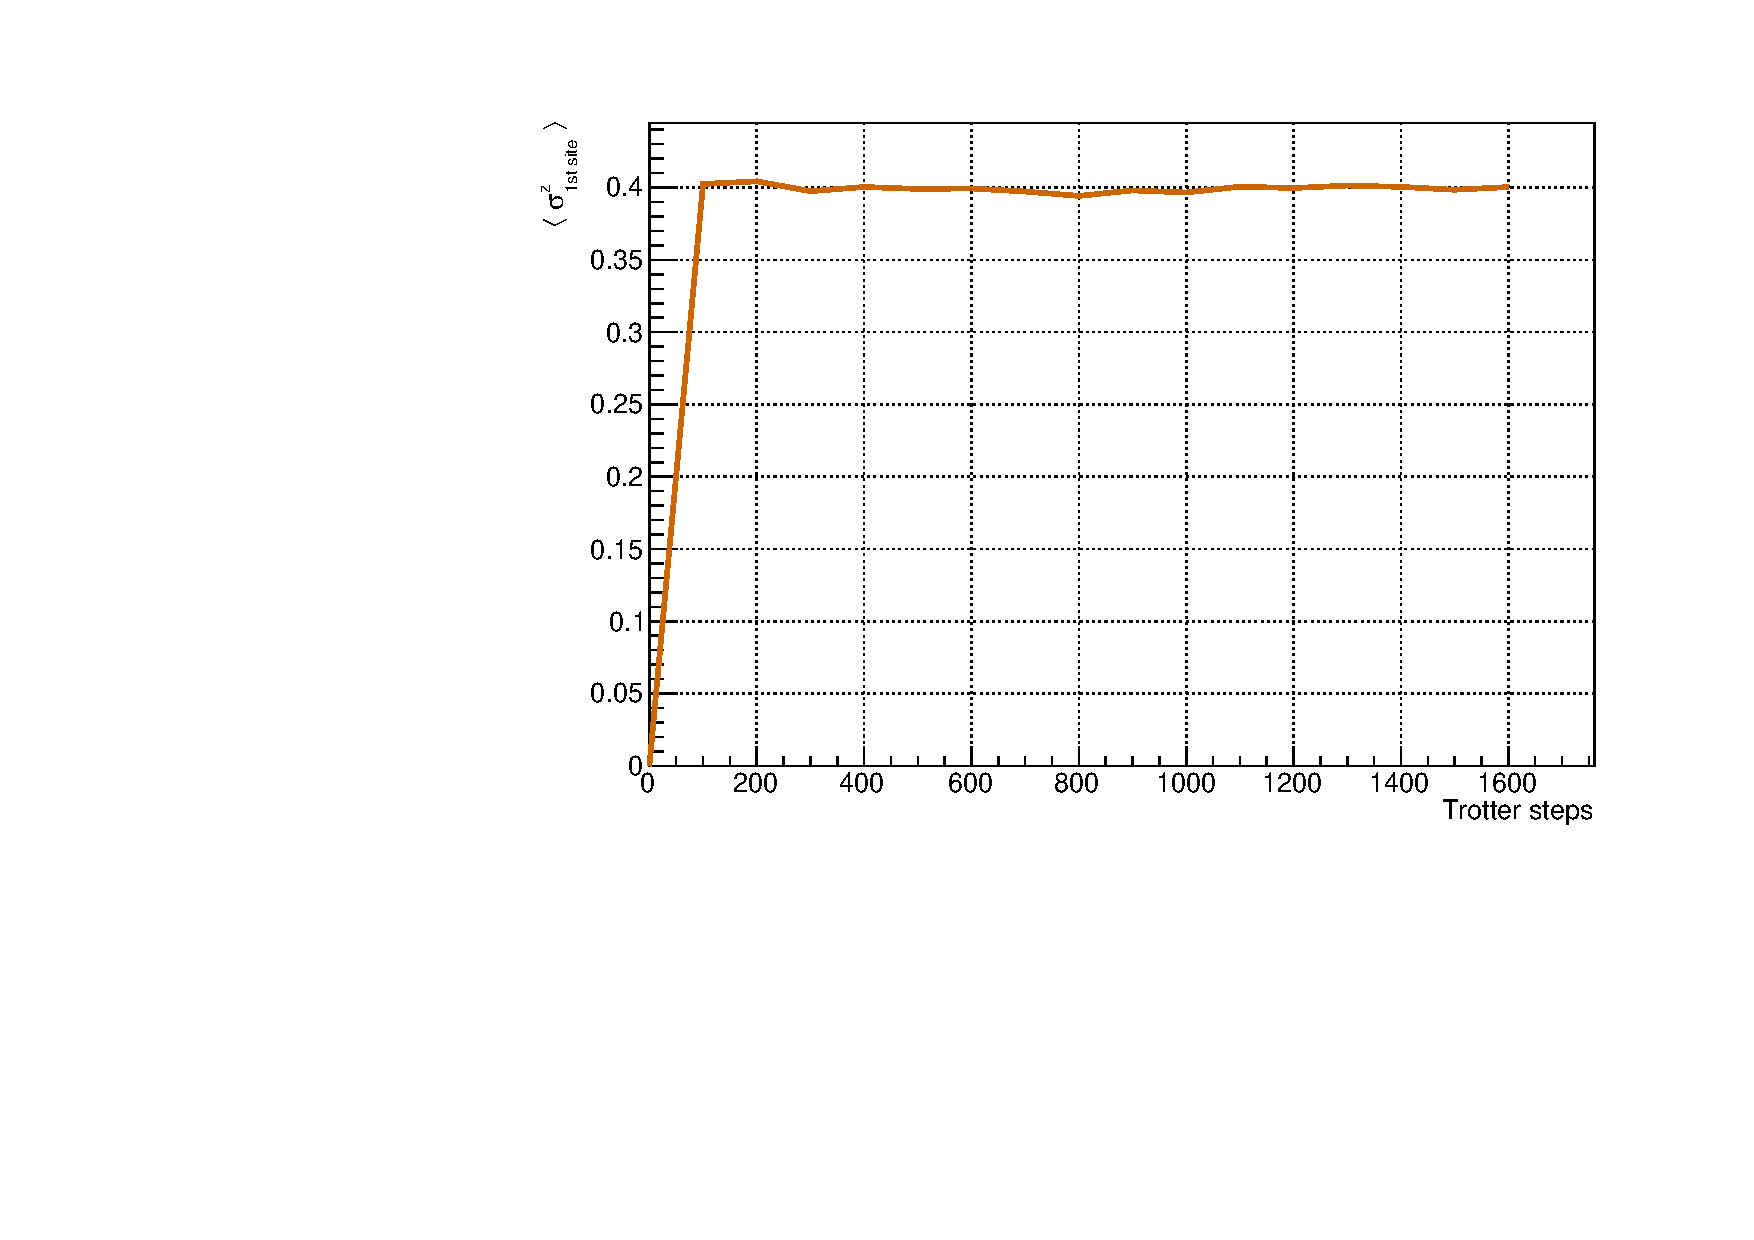
\includegraphics[scale=0.6]{Figures/convergence/Convergence_LM_L012_m060_Time001600_J1051.pdf}
    \label{fig:12sites_LMvsGamma}
\end{subfigure}\\
\begin{subfigure}{\columnwidth}
\centering
    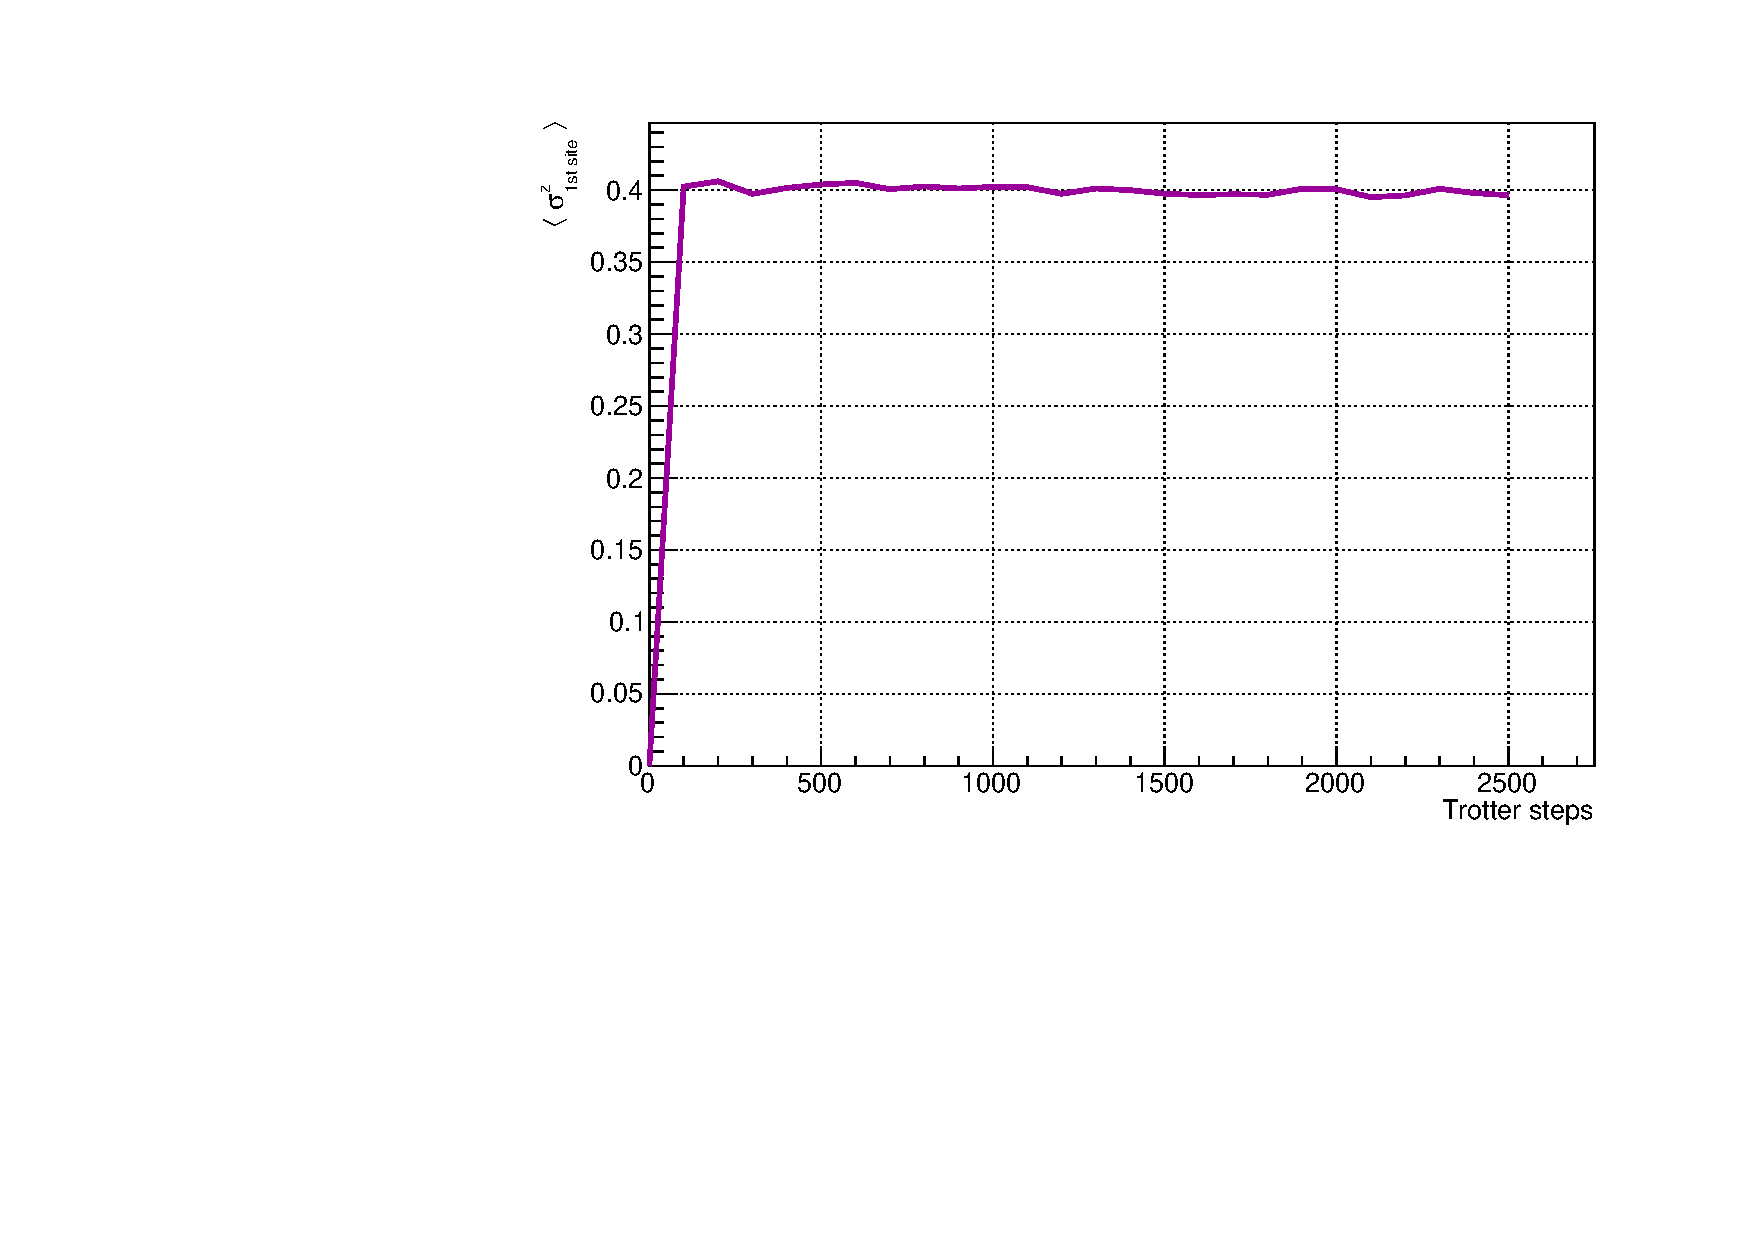
\includegraphics[scale=0.6]{Figures/convergence/ConvergenceLM_L016_m080_Time002500_J1051.pdf}
    \label{fig:16sites_LMvsGamma}
\end{subfigure}\\
\captionsetup{width=1.\linewidth}
\caption{Study of convergence of the MPO method for a 8-sites chain, for bond dimension m = 100 and T = 3000.}
\label{fig:convergence_8_12_16}
\end{figure}

The errors considered for the MPO method are merely the differences between two set of data obtained for two different bond dimension. In particular, the error for an observable $O$ of a 8-sites chain, is given by:
\begin{equation*}
    \epsilon = <O>_{m=100} - <O>_{m=80}.
\end{equation*}